\chapter{Results}
\label{CHAPTER:RESULTS}
\centerline{\rule{149mm}{.02in}}
\vspace{2cm}

\section{Overview}

In this chapter we present the results and analysis of the basic allocation scheme as
implemented in simulation.

\subsection{Auction Implementation}

This section details the single round, sealed bid, first price auction used in
the allocation mechanism. 

The normal flow of a trade is as follows. When a buyer arrives into the system,
it sends an ``advert'' to all its connected sellers.  This advert states the
quantity (job size) of resource which it wishes to purchase. It also sets a
trade time out to occur later, in order to make a decision.

Upon heading an advert, Sellers, check they have the quantity (free resource
capacity) to offer for the Job. If they do, they make an offer (using the basic
ZI-C model as described in section \ref{SEC:ECON:ZI}). If they can not, they
simply ignore the advert.

A Buyer simply records the offers it hears from Sellers, until the trade time out
occurs. It then selects the lowest of all the offers it has heard, and if the
offer's price is below the buyer's limit price, sends an accept message to the
appropriate Seller. 

Upon receiving an accept message from a Buyer, the Seller checks if it is still
able to honour the offer (execute the Job), since it may have accepted other
offers in the meantime, and now be two busy. If it has enough free capacity, it
sends a confirmation to the Buyer and begins executing the Job. When the Buyer
receives the confirmation, it records the successful trade and is removed from
the system.  If the seller can not now honour the original quote, it sends a
cancel message to the Buyer. Upon receiving this, the Buyer removes that quote
from its list, and repeats the acceptance process with next best offer. 

There are some additional factors to handle errors in the trading due to
messages taking too long to arrive. Firstly, when a Buyer sends an accept
message for the lowest offer, it sets an accept time out. If this accept
timeout occurs with out the accepted offer being confirmed by the seller, the
Buyer sends a cancel message to the Seller. When receiving a cancel message
from a Buyer, a Seller can be in one of three states, depending on what
messages it has seen.

\begin{itemize}

  \item The Seller received the accept, but cancelled it as was too busy. The cancel
    message did not arrived before the accept time out occurred for the
    buyer. In this case, the cancel message is ignored. Likewise, when the
    buyer receives the delayed cancel message from the Seller, it is ignored.

  \item The Seller received the accept, sent a confirmation, and started the Job, but
    the confirmation did not arrive in time and the Buyer timed out and
    cancelled. In this case the Seller cancels the running Job. The
    confirmation, when it arrives at the buyer is ignored.

  \item The Seller did not receive the original accept message, so never
    responded, and ignores cancellation message.

\end{itemize}

If the Buyer has no valid offers when a trade time out occurs, it sets another
trade time out to wait for more offers to arrive. The number of time outs a
Buyer can set is limited, and if this limit is reached and no valid offers have
been heard or accepted, the Buyer reports failure and is removed from the
system.

Table \ref{TABLE:RESULTS:PARAMS} shows the various parameters used in
implementing this auction mechanism.

\begin{table}
  \begin{center}
    \begin{tabular}{| l | c |}
      \hline
      Description & Value \\ 
      \hline
      Max. trade time outs	      & 5 \\
      Trade time out delta     & 3s \\
      Accept time out	delta     & 8s \\
      Minimum price     & \$0.01 \\
      Maximum price     & \$10.00 \\
      \hline
    \end{tabular}
  \end{center}

  \caption{Parameter values for the sealed auction mechanism}
  \label{TABLE:RESULTS:PARAMS}
\end{table}

\subsection{Network Topology}

The base network type is a random network. It constructed from three
parameters, network size, mean degree and a minimum degree. First the total
number of links is calculated from the network size and mean degree. Then each
node is given the minimum degree number of links to other random nodes. Other
links are added between two random nodes until the total number of links has
been allocated created. The use of minimum degree is designed to skew the
distribution of degree slightly to make sure traders have a viable number of
other traders with which to trade.

The values used for the above parameters for the base random network were
determined through experimentation, and the results of which are presented in
Appendix \ref{CHAPTER:APPENDIX}. A mean degree of 128 chosen to maximise the
connectedness of the network, whilst still being able to cope with the
communication costs on a system with a load of 2.0.

All results presented here are the average of 10 simulation runs.

\section{Base System Performance}

\begin{figure}[h] 
  \centering
  \fbox{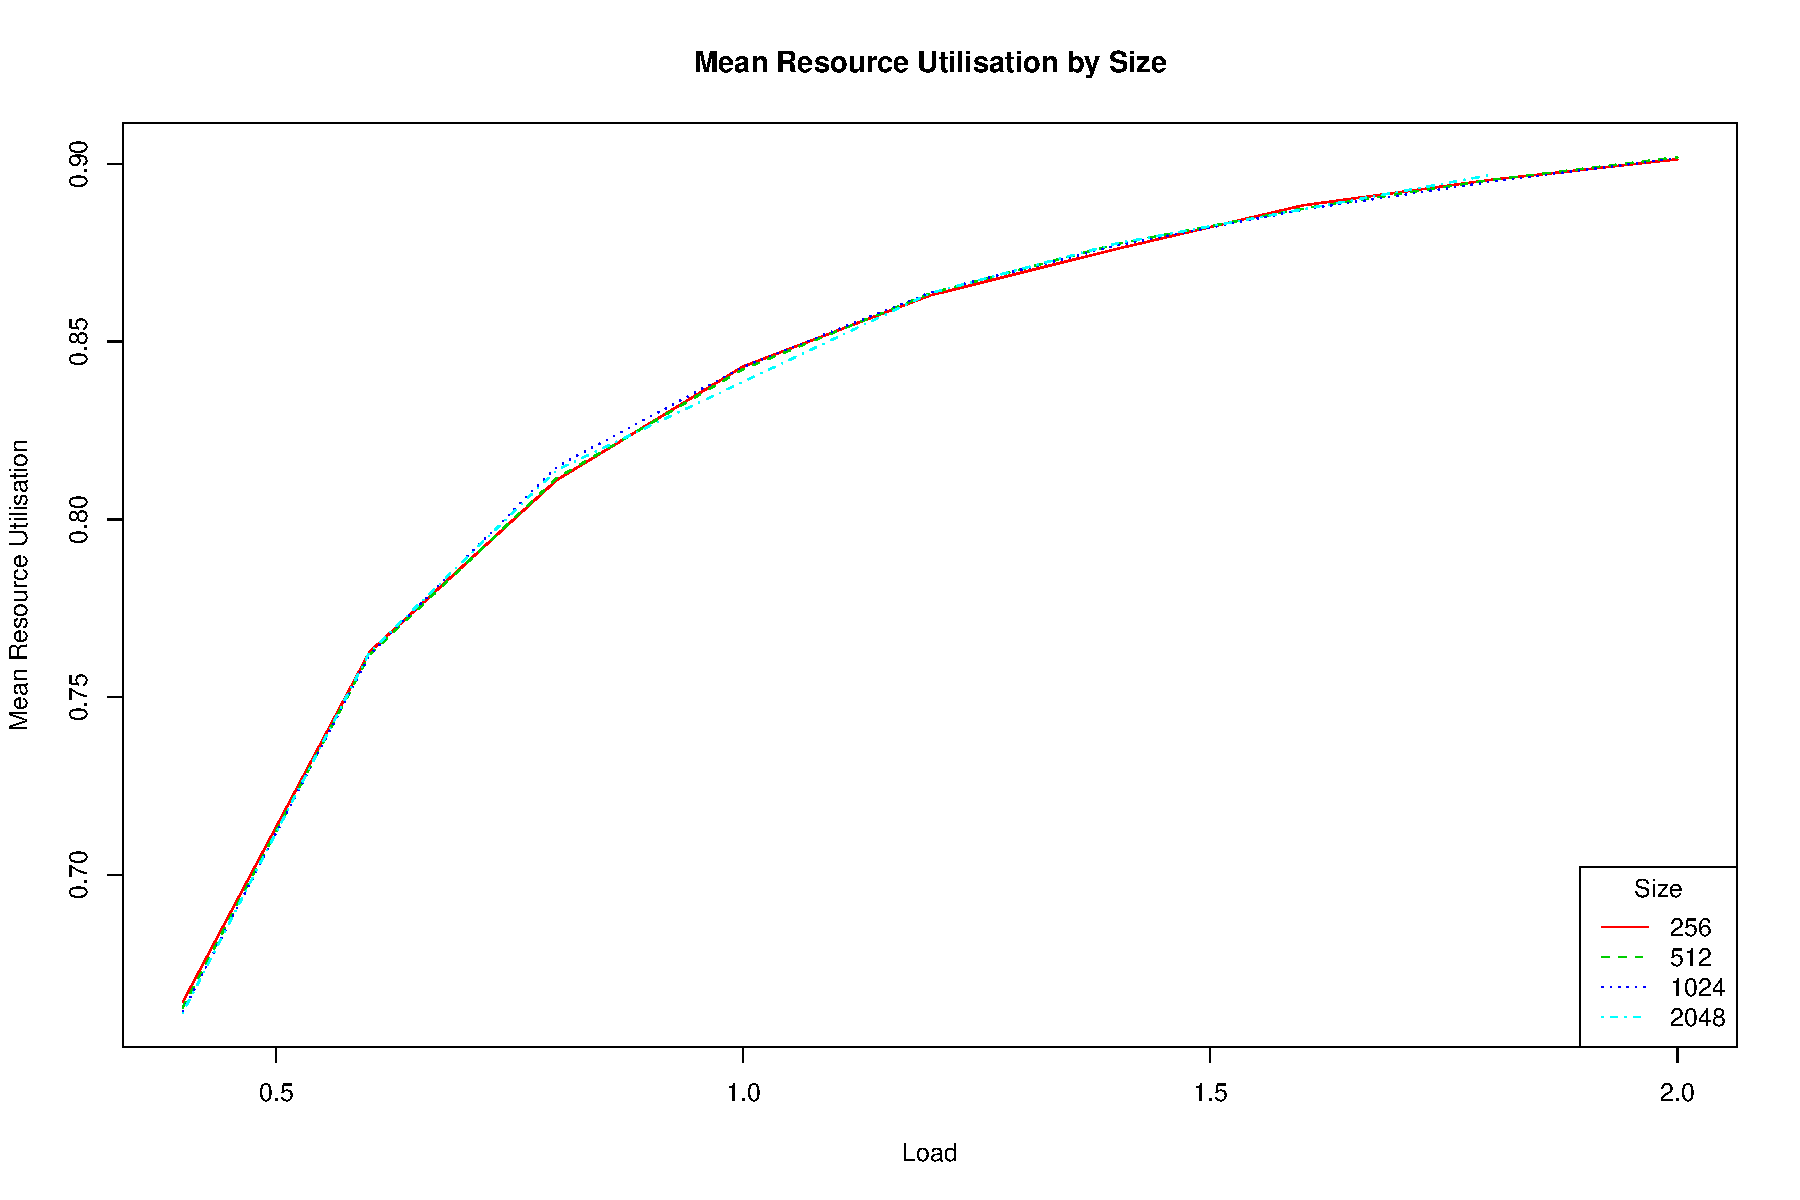
\includegraphics[width=14cm]{results/resource_util_mean}}
  
  \caption{The mean resource utilisation for the system against load and size.
  This shows the scalability of the system, as there is no significant
  difference between network sizes. At a load of 1.0, where an optimal
  allocation would achieve close to 100\%, the system achieves about
  80\% utilisation.}

  \label{FIG:RES:RUTIL}
\end{figure}

\begin{figure}[h] 
  \centering
  \fbox{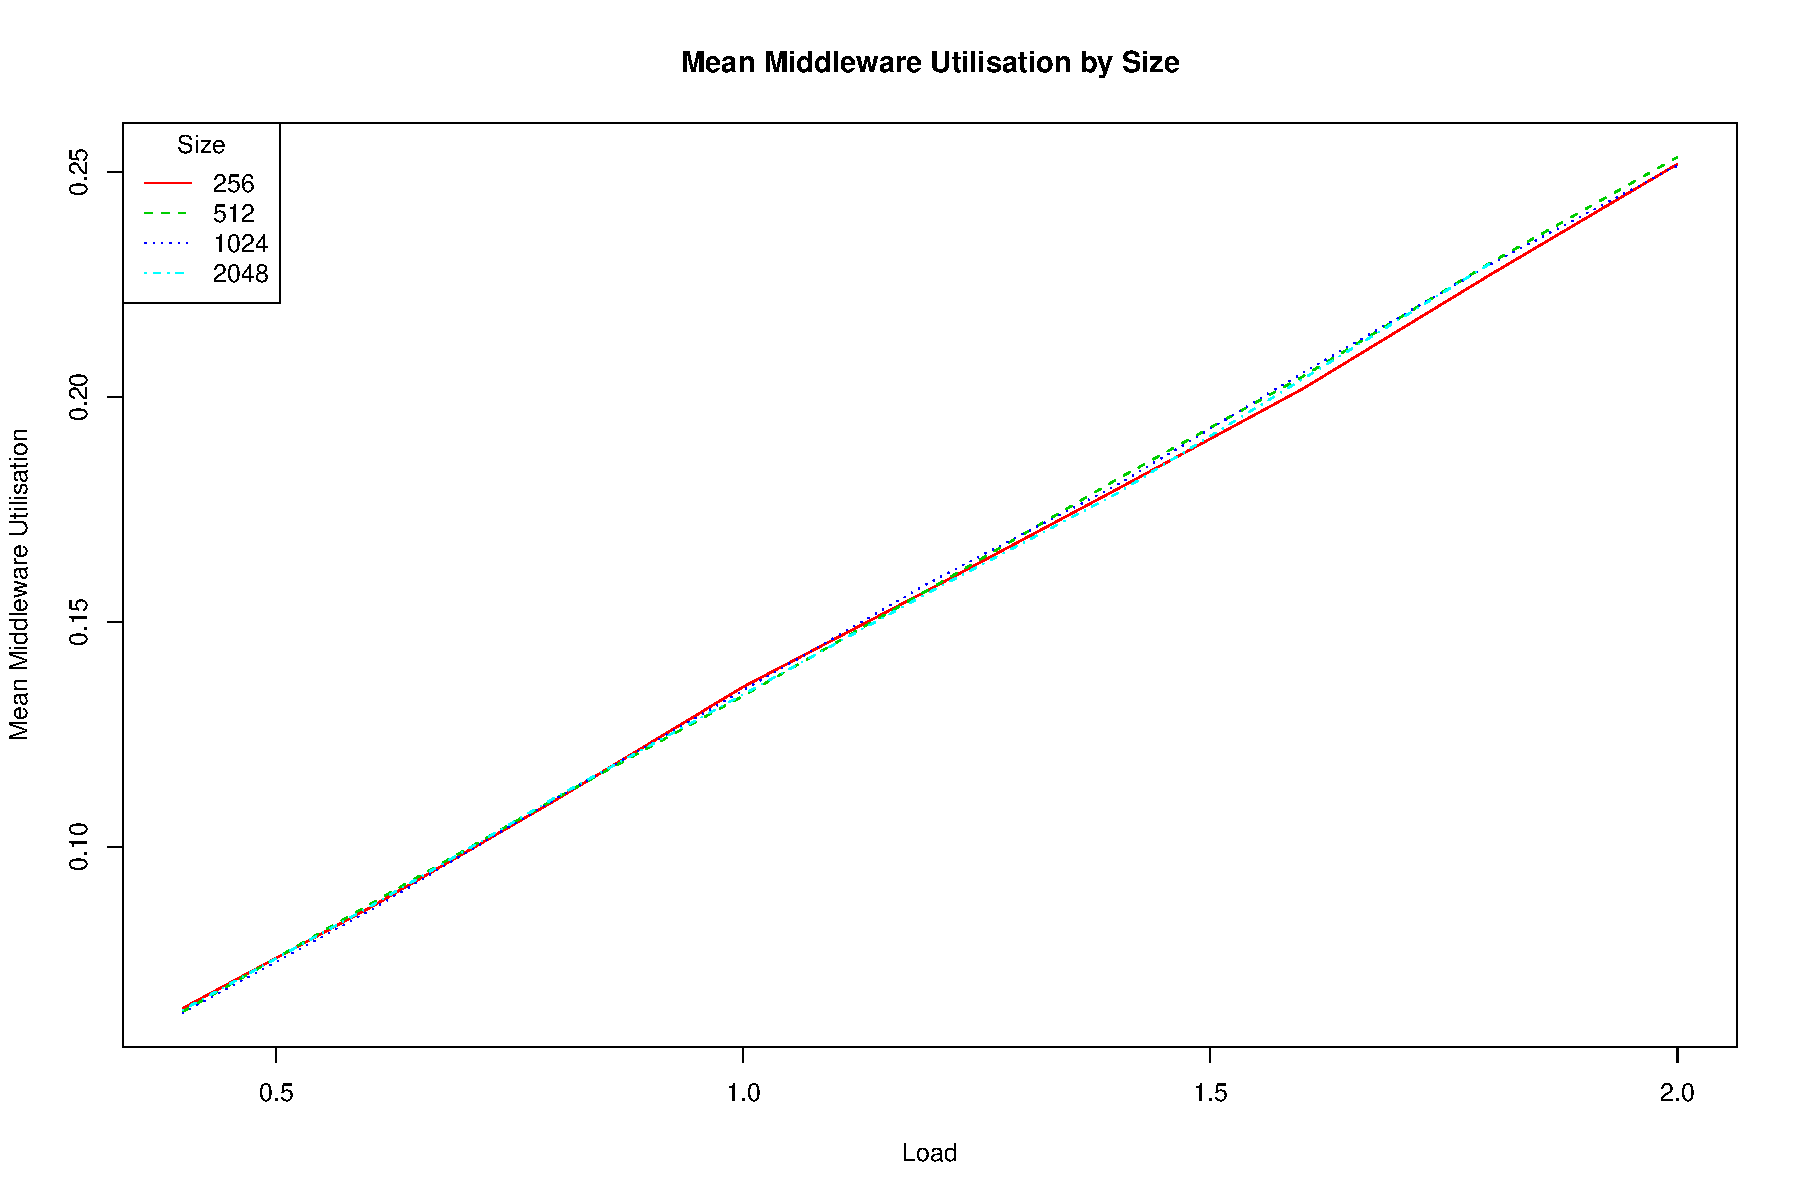
\includegraphics[width=14cm]{results/middleware_util_mean}}

  \caption{The mean middleware utilisation for the system against load and
  size. The middleware utilisation does not rise above 25\% and is easily able
  to handle the communication load. Again size has now impact and the
  utilisation is a linearly related to the number of Jobs in the system}

  \label{FIG:RES:MUTIL}
\end{figure}

\begin{figure}[h] 
  \centering
  \fbox{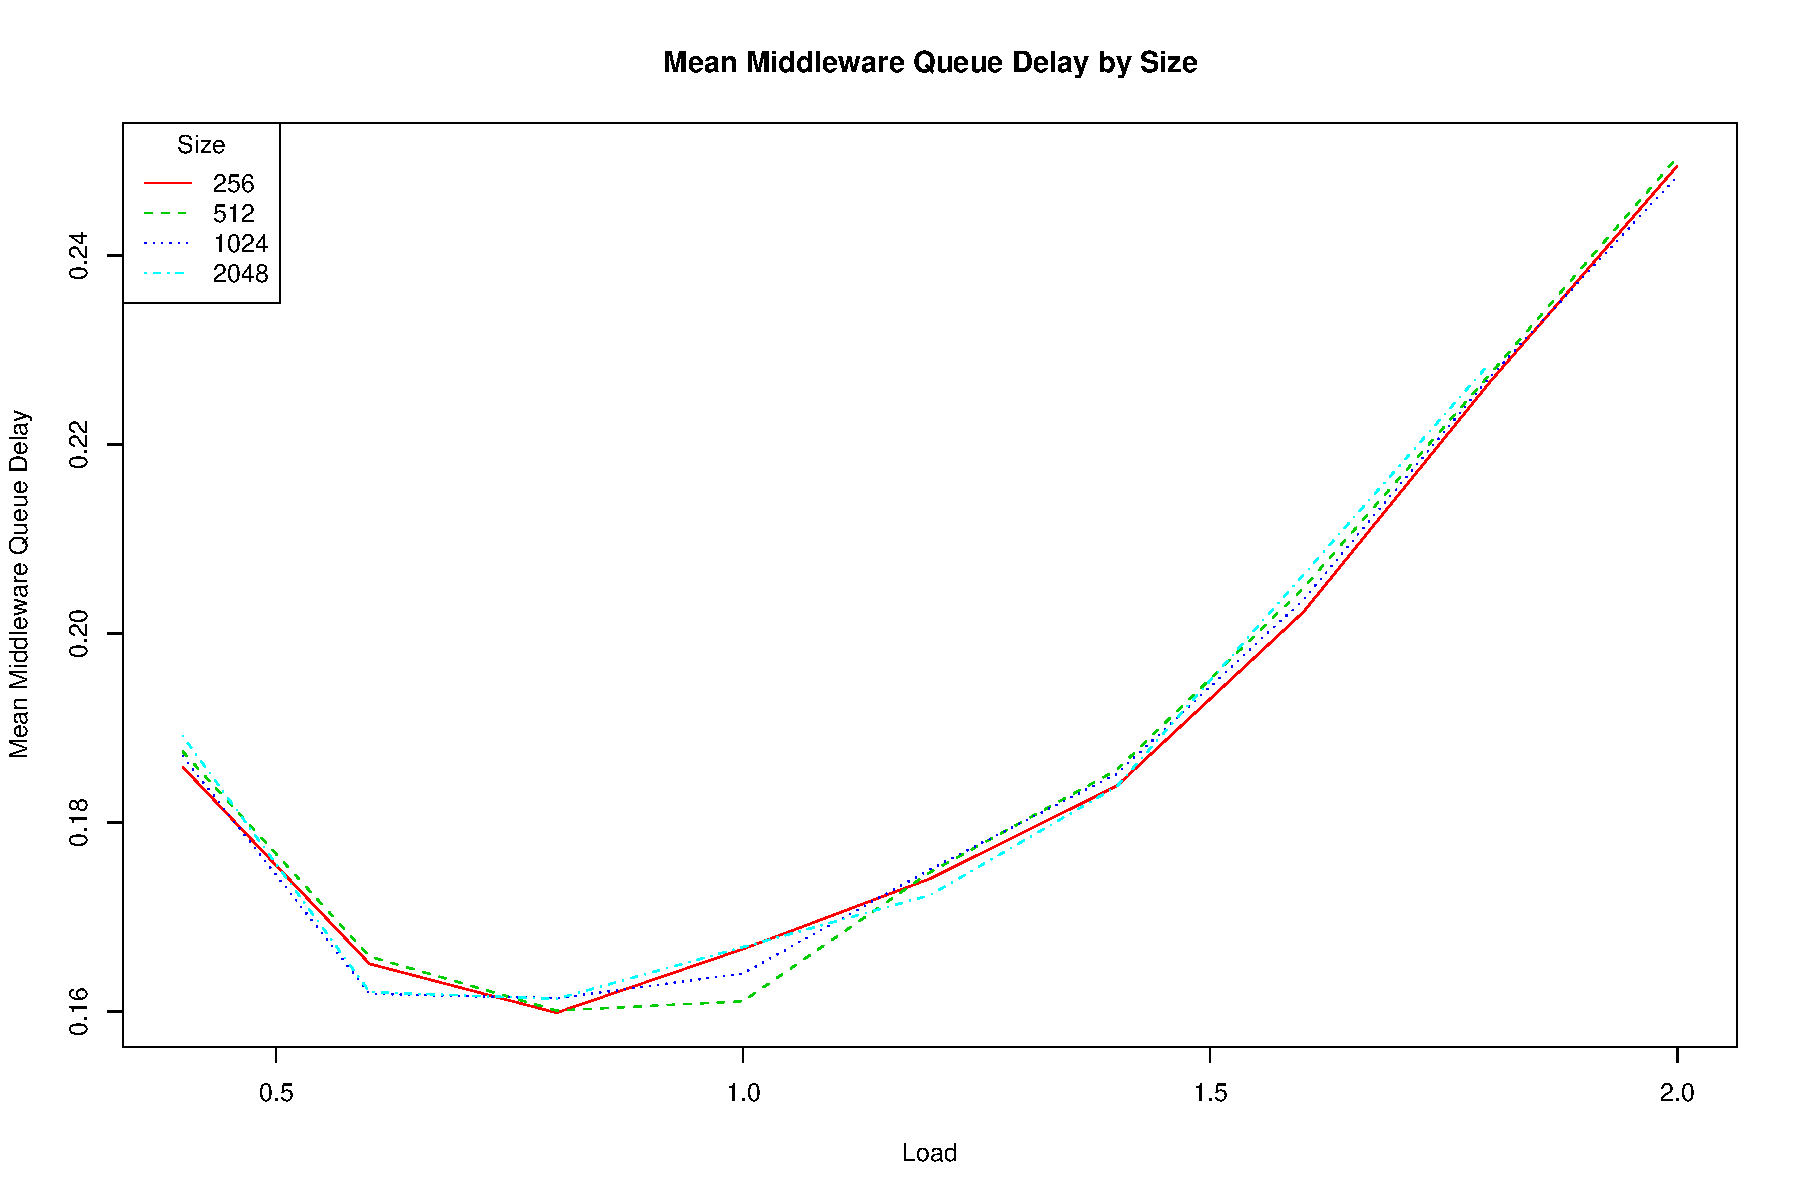
\includegraphics[width=14cm]{results/queue_delay_mean}}

  \caption{The mean delay of a message due to the queuing to be served by the
  middleware, against load and size.  Again note the lack of impact of the
  network size. The higher delay at the start is an anomalous result, but is
  only a very small of about 0.03s. This suggests that its is an insignificant
  artefact of the simulation when run with low loads.}

  \label{FIG:RES:QDELAY}
\end{figure}


\begin{figure}[h] 
  \centering
  \fbox{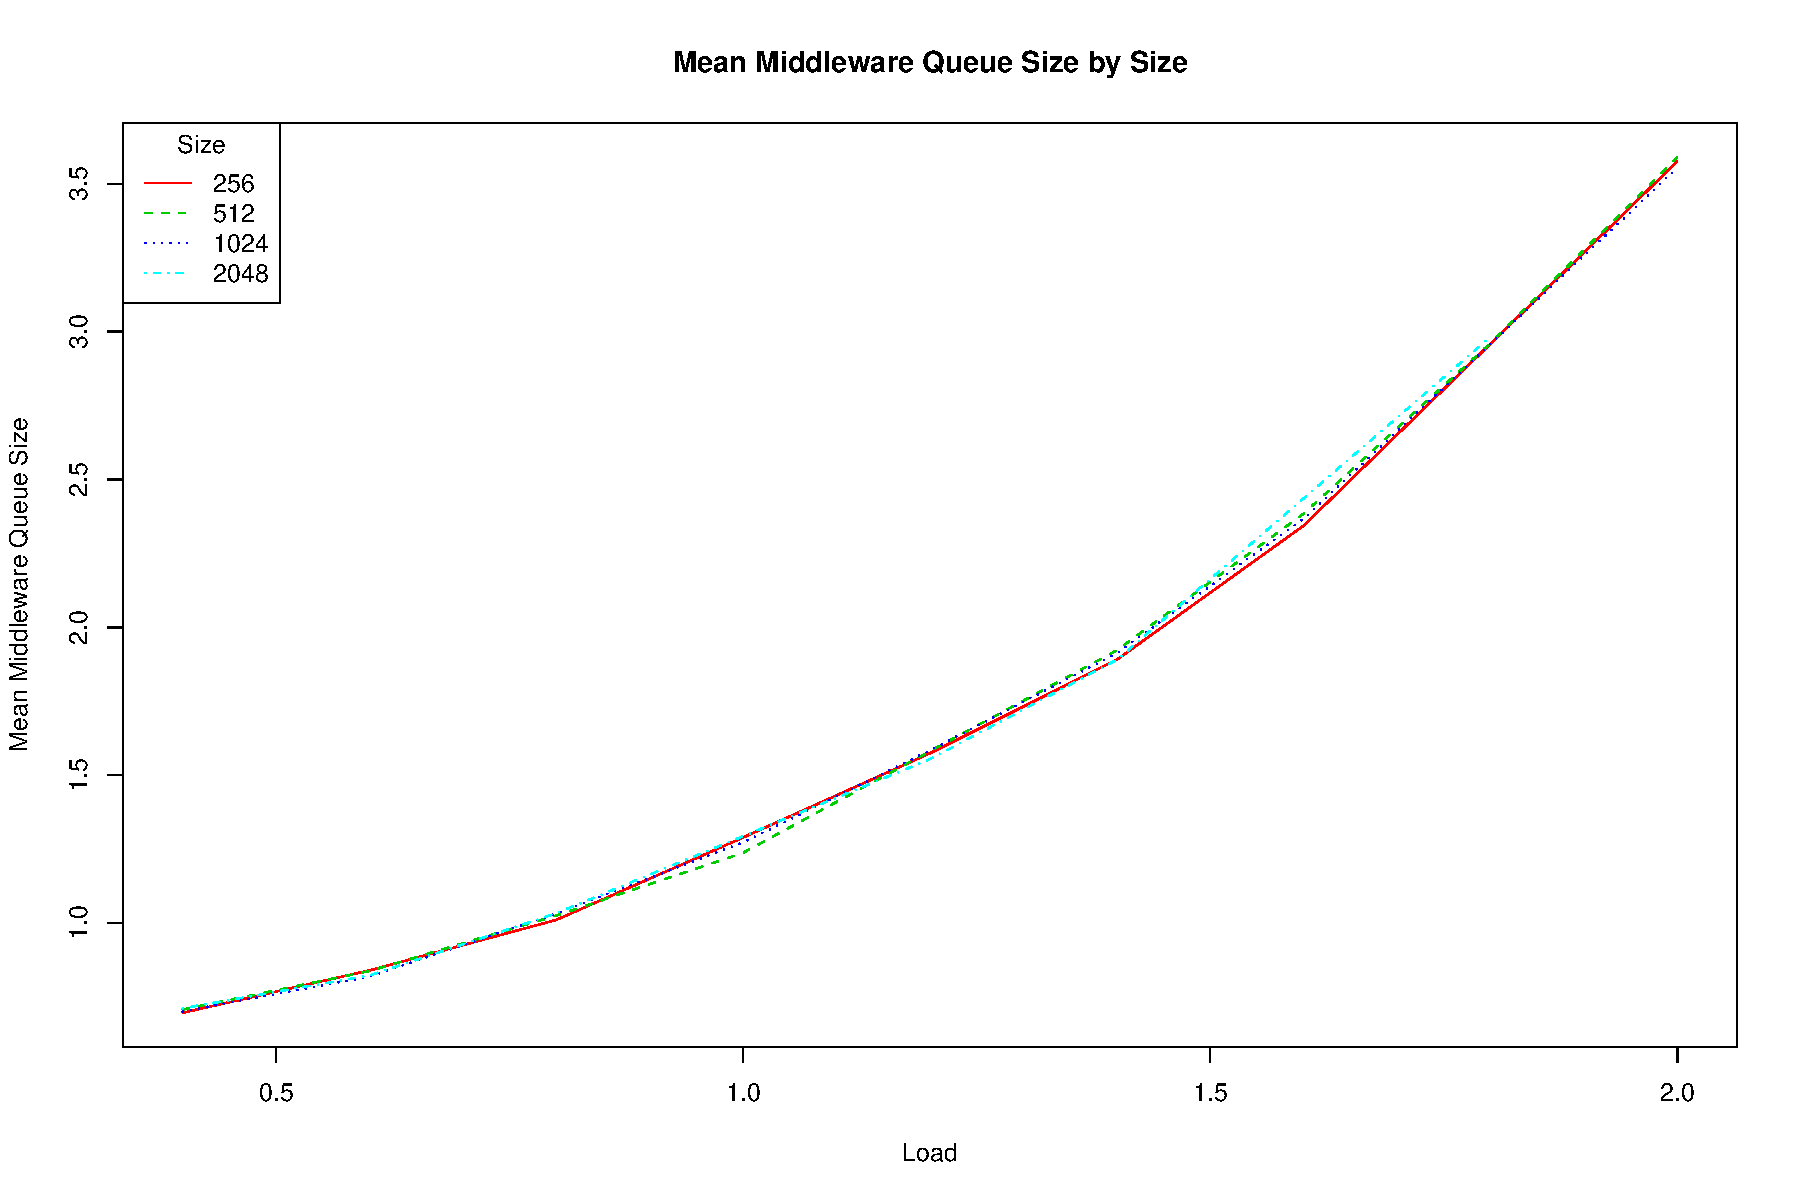
\includegraphics[width=14cm]{results/queue_size_mean}}

  \caption{The mean middleware message queue size. This is not affected by size
  an gives and indication of the level of concurrent required by the
  middleware.}

  \label{FIG:RES:QSIZE}
\end{figure}

\begin{figure}[h] 
  \centering
  \fbox{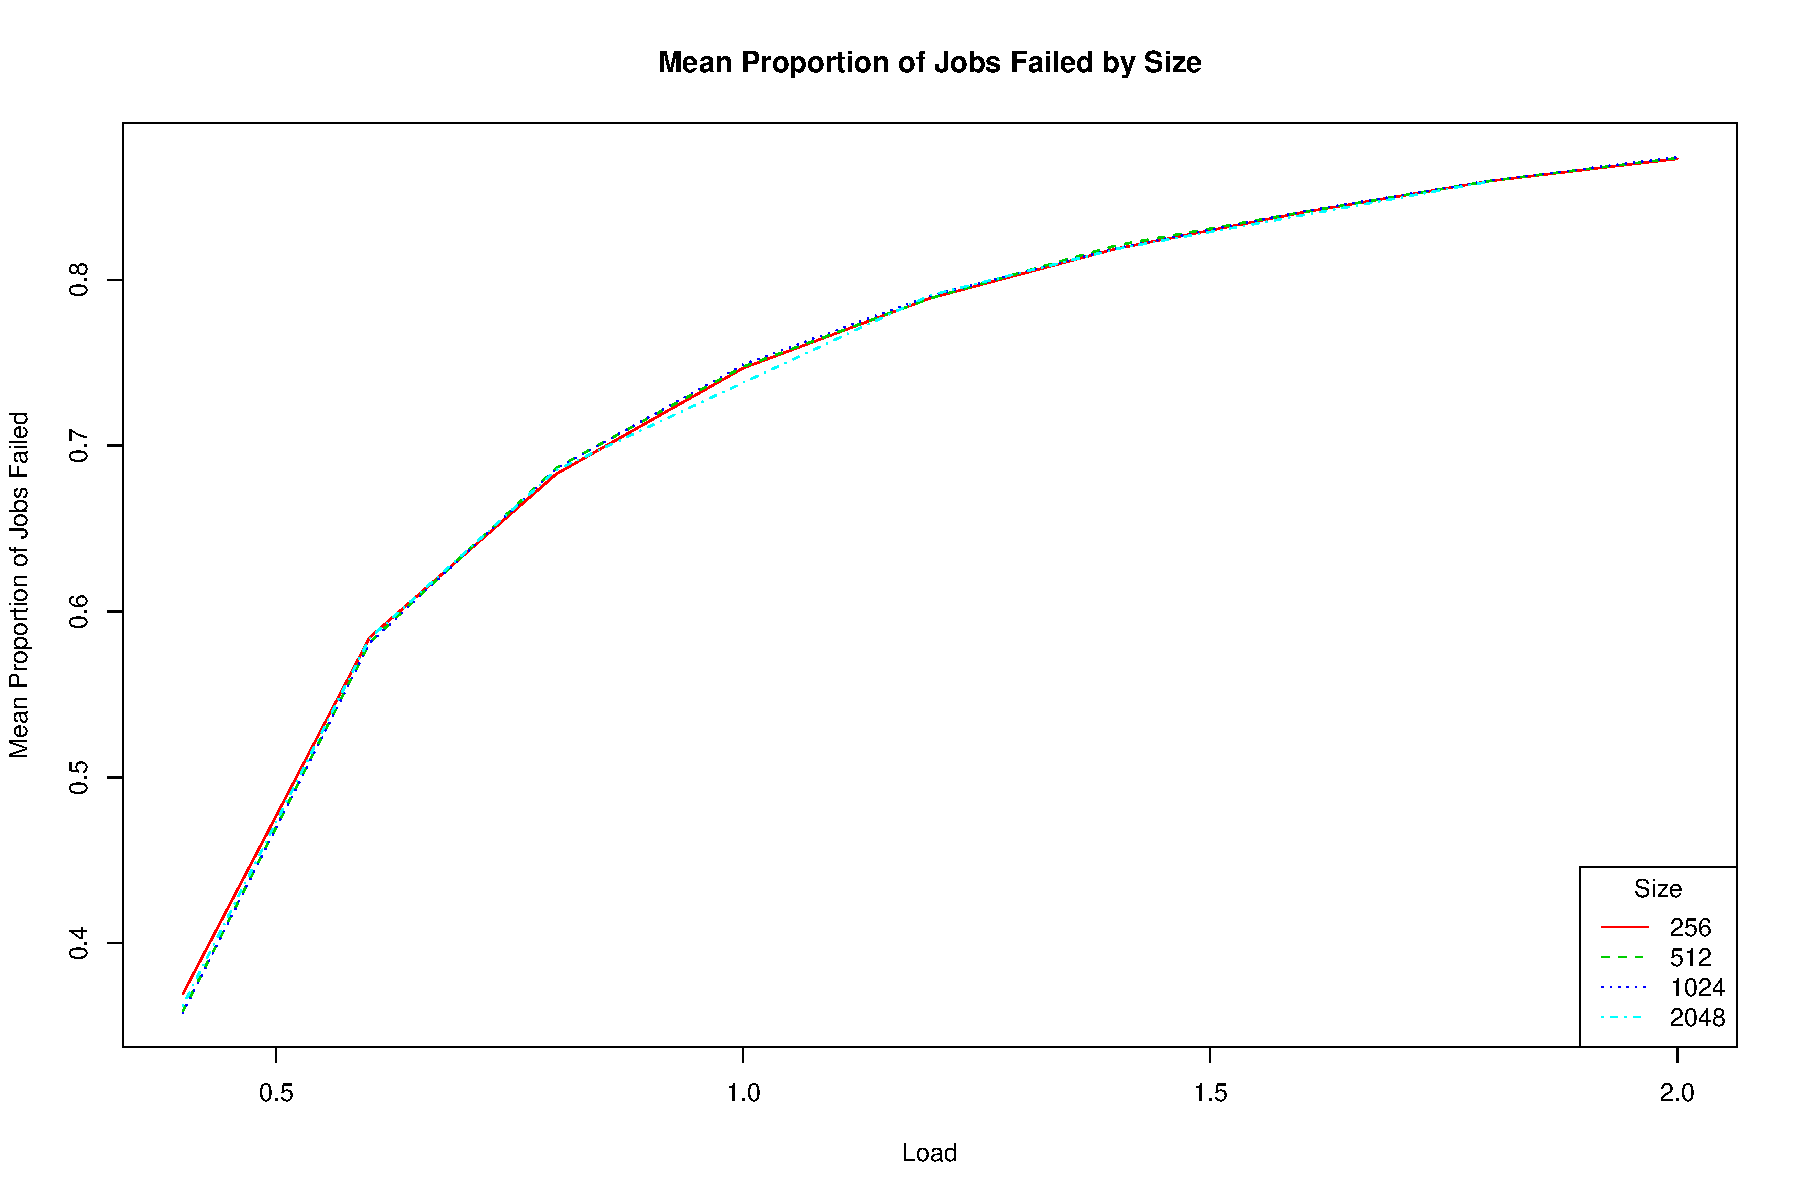
\includegraphics[width=14cm]{results/prop_failed}}
  \caption{The proportion of jobs that failed to allocate.}
  \label{FIG:RES:PROPFAILED}
\end{figure}

\begin{figure}[h] 
  \centering
  \fbox{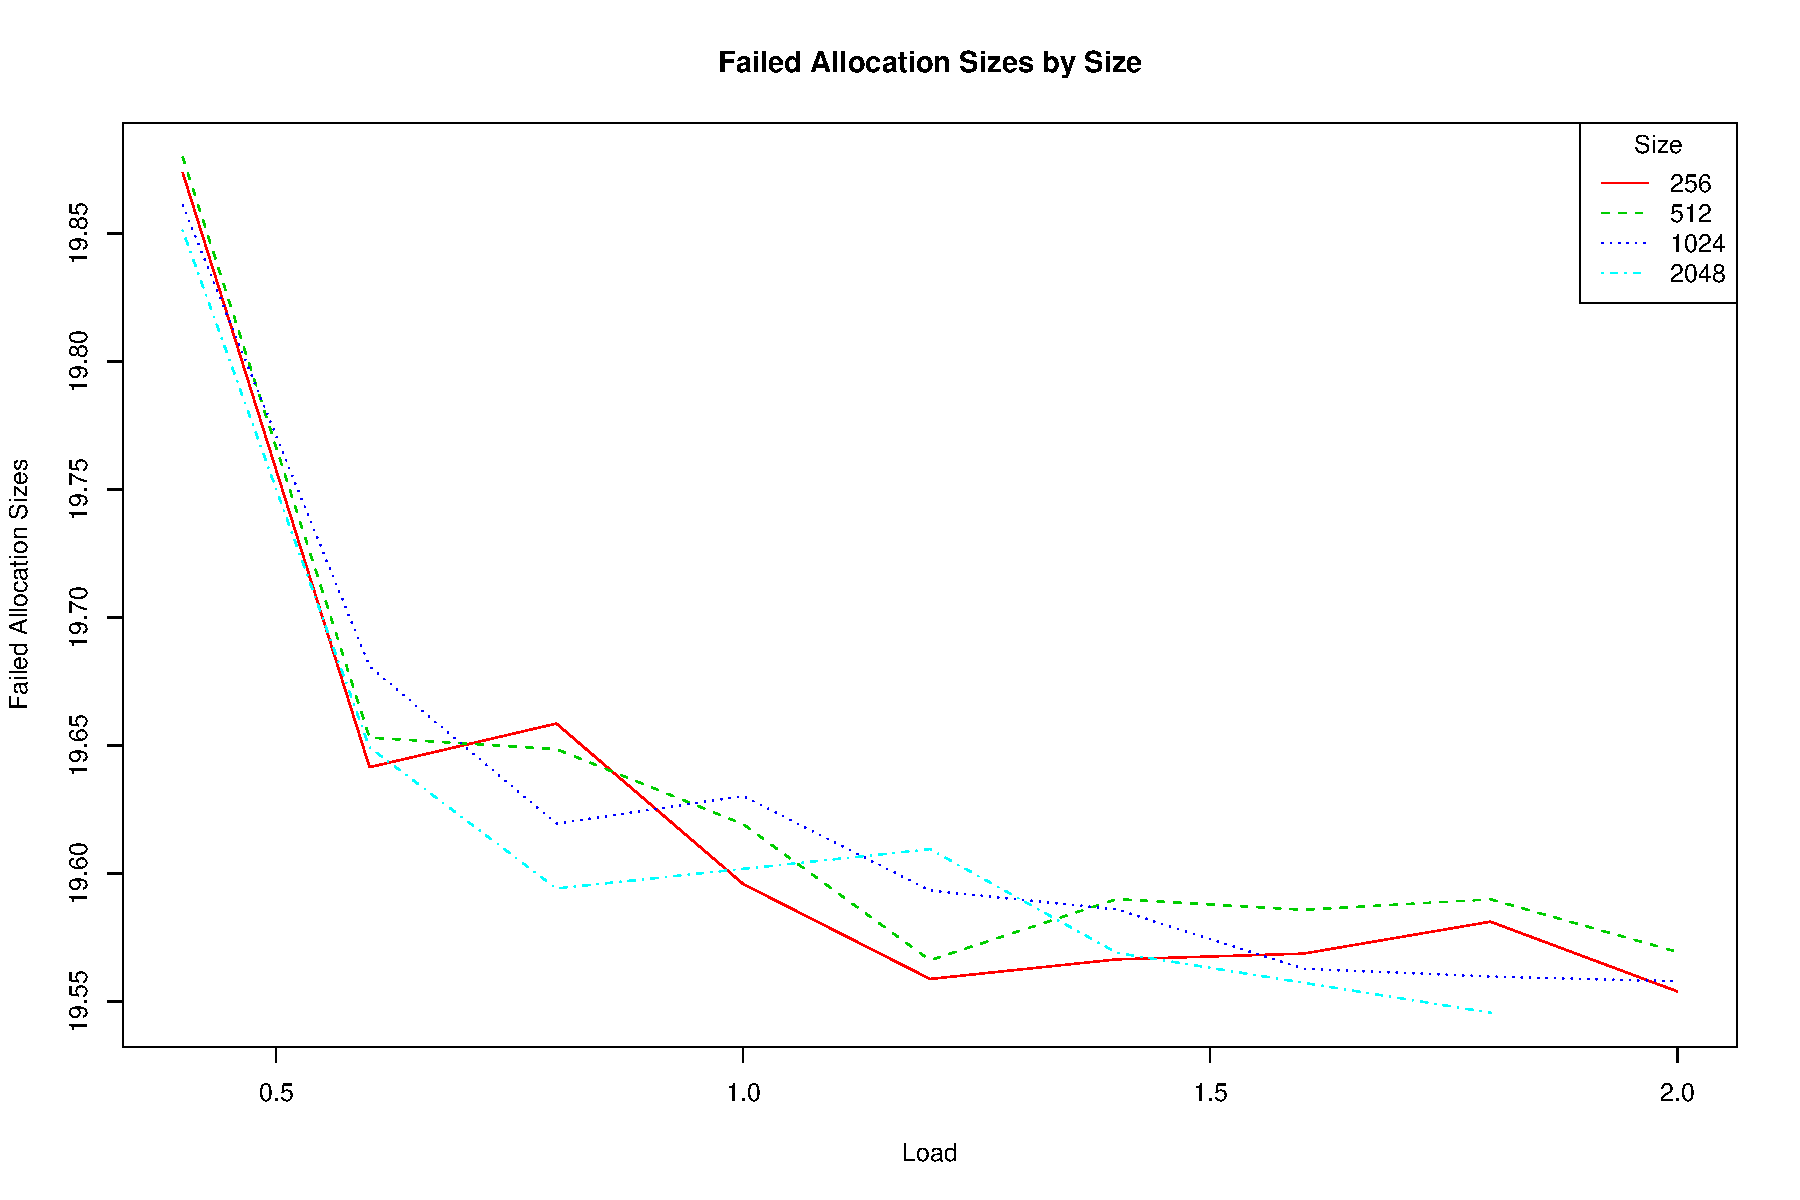
\includegraphics[width=14cm]{results/failed_sizes_mean}}
  \caption{The mean size of jobs that failed to allocated.}
  \label{FIG:RES:FAILEDSIZES}
\end{figure}

\begin{figure}[h] 
  \centering
  \fbox{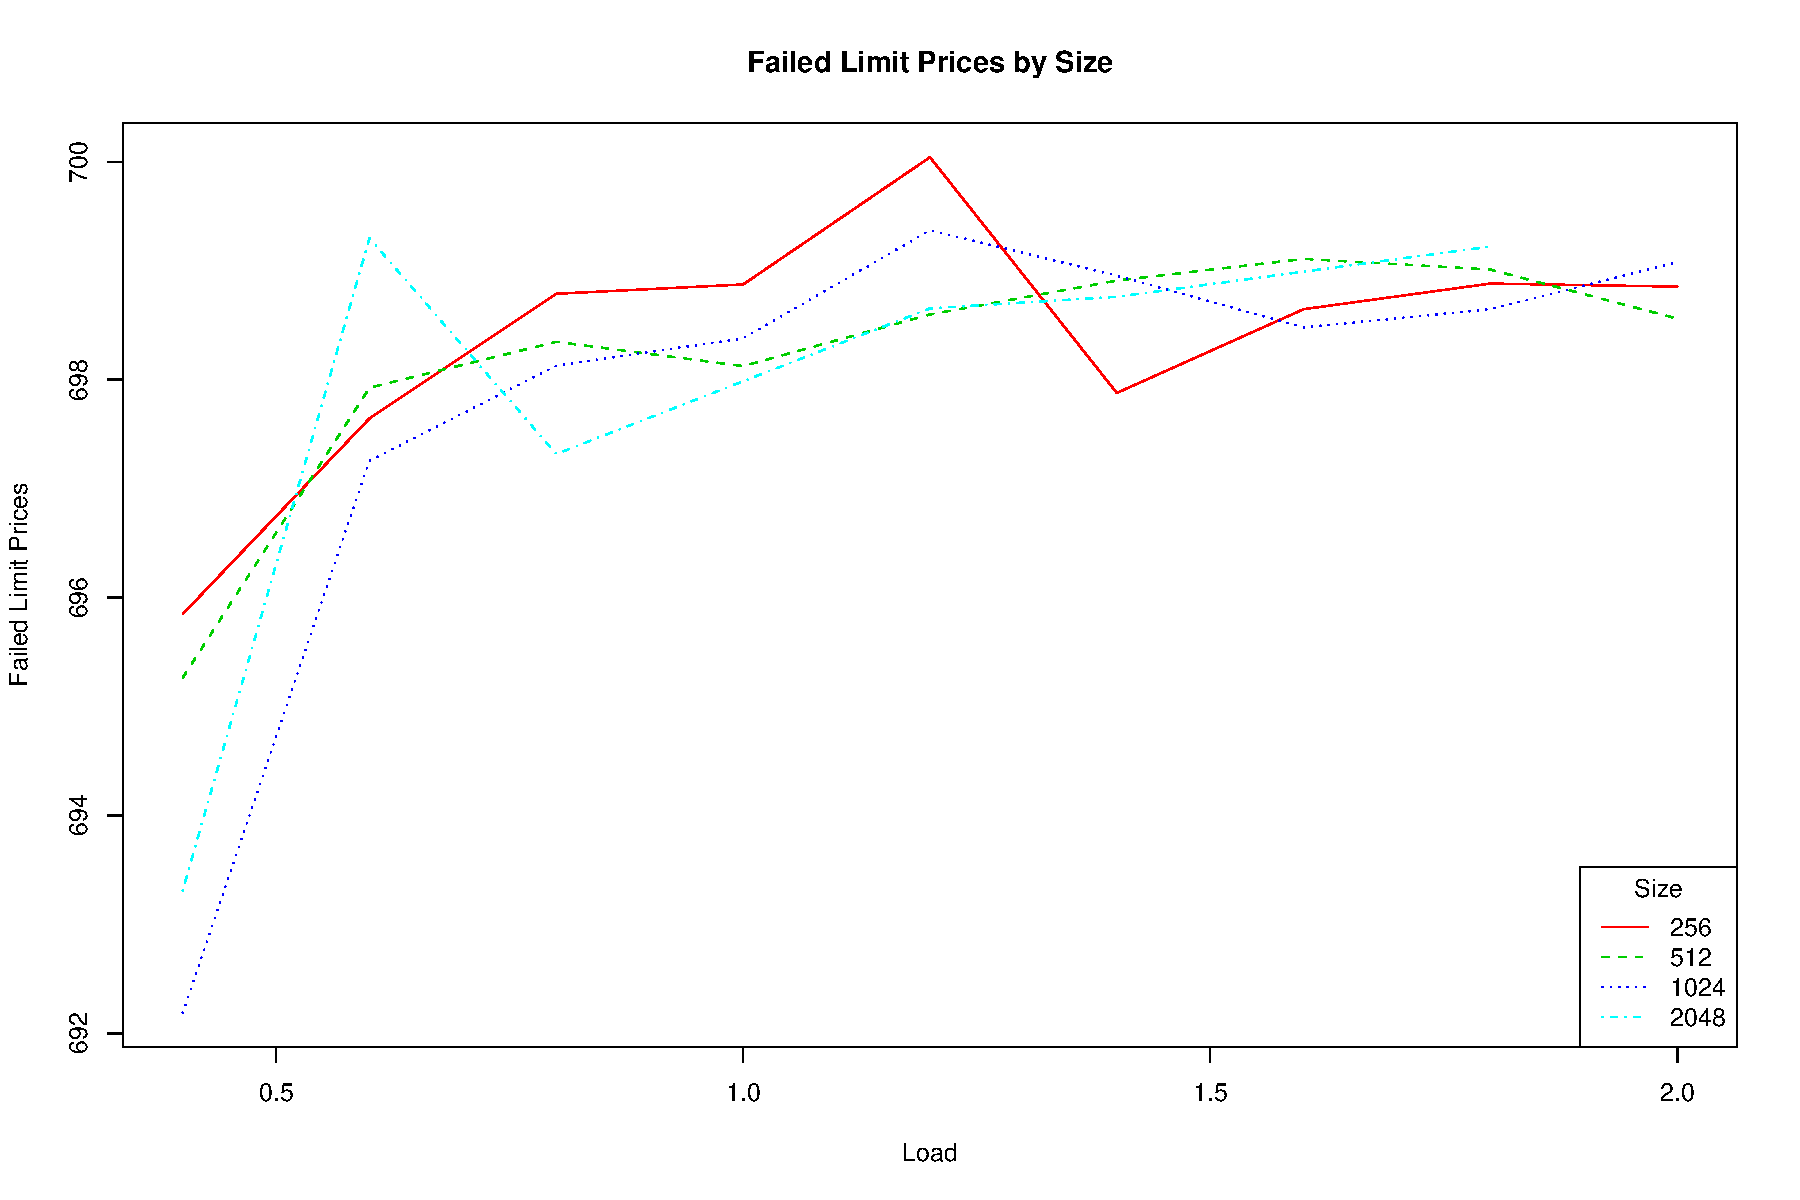
\includegraphics[width=14cm]{results/failed_limit_prices_mean}}
  \caption{The mean limit price of Buyers who failed to allocate their Jobs}
  \label{FIG:RES:FAILEDLIMITS}
\end{figure}

\begin{figure}[h] 
  \centering
  \fbox{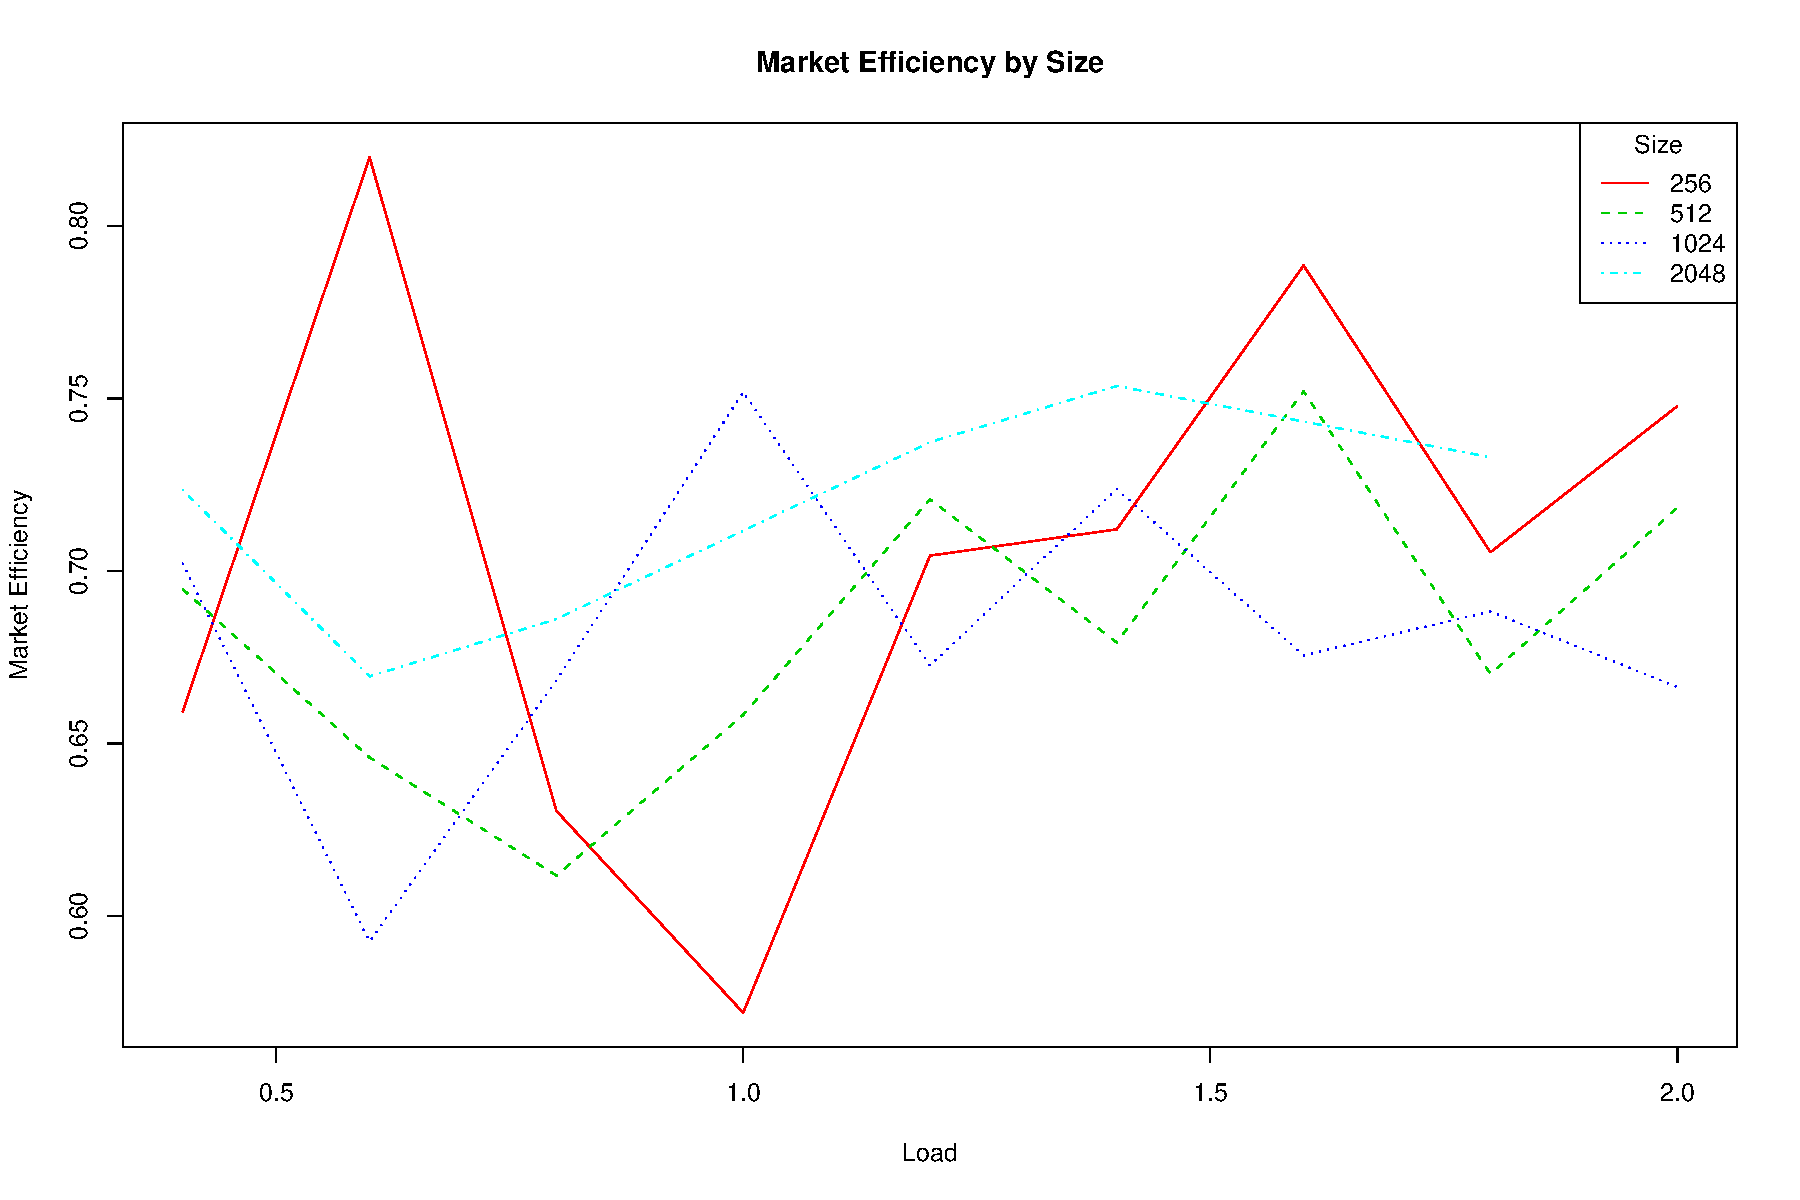
\includegraphics[width=14cm]{results/efficiency}}
  \caption{The mean efficiency of the ZI/sealed bid marketplace.}
  \label{FIG:RES:EFFICIENCY}
\end{figure}


Figures \ref{FIG:RES:RUTIL}, \ref{FIG:RES:MUTIL}, \ref{FIG:RES:QDELAY} and 
\ref{FIG:RES:QSIZE} show the utilisation of the modelled hardware
resources on the grid, both the resources themselves and the middleware system
used to model communication. The plots show the various utilisation statistics
of the system against system load and system.

The key result demonstrated by all the results in this section is the high
scalability of the system.  The size has no effect at on the base performance of
the system. This clearly demonstrates the potential benefits of a decentralised
system.  Given the lack of effect of size as a system parameter, a standard
size of 1024 nodes is used for other further experiments.

The simulated middleware system's performance is easily able to cope with the
level of traffic created by the traders, which is encouraging given we chose to
give them only modest performance metrics.



Whilst the base grid system performs well and scales excellently, the system is
only moderately successful at allocating jobs. Figure \ref{FIG:RES:PROPFAILED}
shows the proportion of jobs that failed to be successfully allocated, which is
significantly large. 


An allocation can fail for two reasons. The first arises from the constraints
from our grid model, which requires that the desired quantity (Job size) is not
divisible. As in any economic system where this is the case, when the system
resources are close to fully allocated,  Buyers may not be able to buy enough
quantity of non-divisible resource at all.  Figure \ref{FIG:RES:FAILEDSIZES}
shows the mean size of jobs that failed to allocate.  While smaller Job sizes
were more successful under higher load, the variation is small, and this is
unlikely to be the significant factor in the high proportion of failed jobs.

The second reason that an allocation can fail in our system the variance in
limit prices could mean a Buyer with a low limit price can receive no
offers below their limit. However, figure \ref{FIG:RES:FAILEDLIMITS} shows
that there was very little variation in failed limit prices.

However, the above factors do not seem to play a significant part in high
proportion of failed allocations. Therefore, the key factor in this behaviour
is that traders only have local knowledge, so not all Buyer can advertise to
all Sellers, nor can Sellers offer on all Jobs.  This means that while there
may be a Seller and Buyer in the system who are able to trade, there is no link
between them and therefore the allocation fails. This suggests that mean degree
is a key factor in these experiments.

The efficiency of the market is shown in figure \ref{FIG:RES:EFFICIENCY}. The
results are similar to the original ZI work, in that there is measure of
efficiency, but it is not consistent.

\subsection{Summary}

The basic results indicate that system provides a trade off between an
efficient allocation and a scalable allocation.  A high degree of scalability
is achieved at the cost of a significantly less than optimal allocation. 


\section{Network Topologies}

\subsection{Implementation Details}
\label{SEC:RESULTS:NETWORKS}

Two topologies were investigated, a small world topology and a scale-free one.
The creation of the small world was implemented in the same manner as in
\cite{net-watts98-smallworld}. That is, the nodes are arranged in a ring
structure, with the idea that the closer you are to another node on the ring,
the more 'local' that node is to you. In a similar fashion to the generation of
the random network, links are added until the total number of links is reached.
However, in a small world network, each is by default local, connected to the
nearest unconnected node along the ring. The link can instead be a global one
based on a probability $p$. A global link is between two random nodes, and
represents the long distance links that give rise to small world properties.

The algorithm used for creating a scale-free network is the preferential
attachment algorithm proposed in \cite{net-barabasi99-scaling}. Each is node is
given the minimum number of links, as with the random topology. The rest of the
links are added randomly, but with a preference for connecting to highly
connected nodes. The degree at which a node prefers to connect to a particular
node is expressed as an exponent of the number of links that node has. Thus an
exponent of zero means no preference and is essentially a normal random
network, where an exponent of two expresses a high preference from linking to
``popular'' nodes. A roulette selection process is used to select nodes to link
to.


%The social network inspired topology uses a novel approach to constructing
%networks. As in the random topology, each node is given the minimum number of
%links. A two unlinked random nodes are chosen and linked together, after which
%a number of friend-of-a-friend (FOAF) links are added by selecting a link from
%one node that the other does not have, and linking that to the other. These
%FOAF links close a triangle between the newly linked nodes, and thus gives rise
%to a high clustering coefficient, similar to real world social networks.

\subsection{Performance}

\begin{figure}[h] 
  \centering
  \fbox{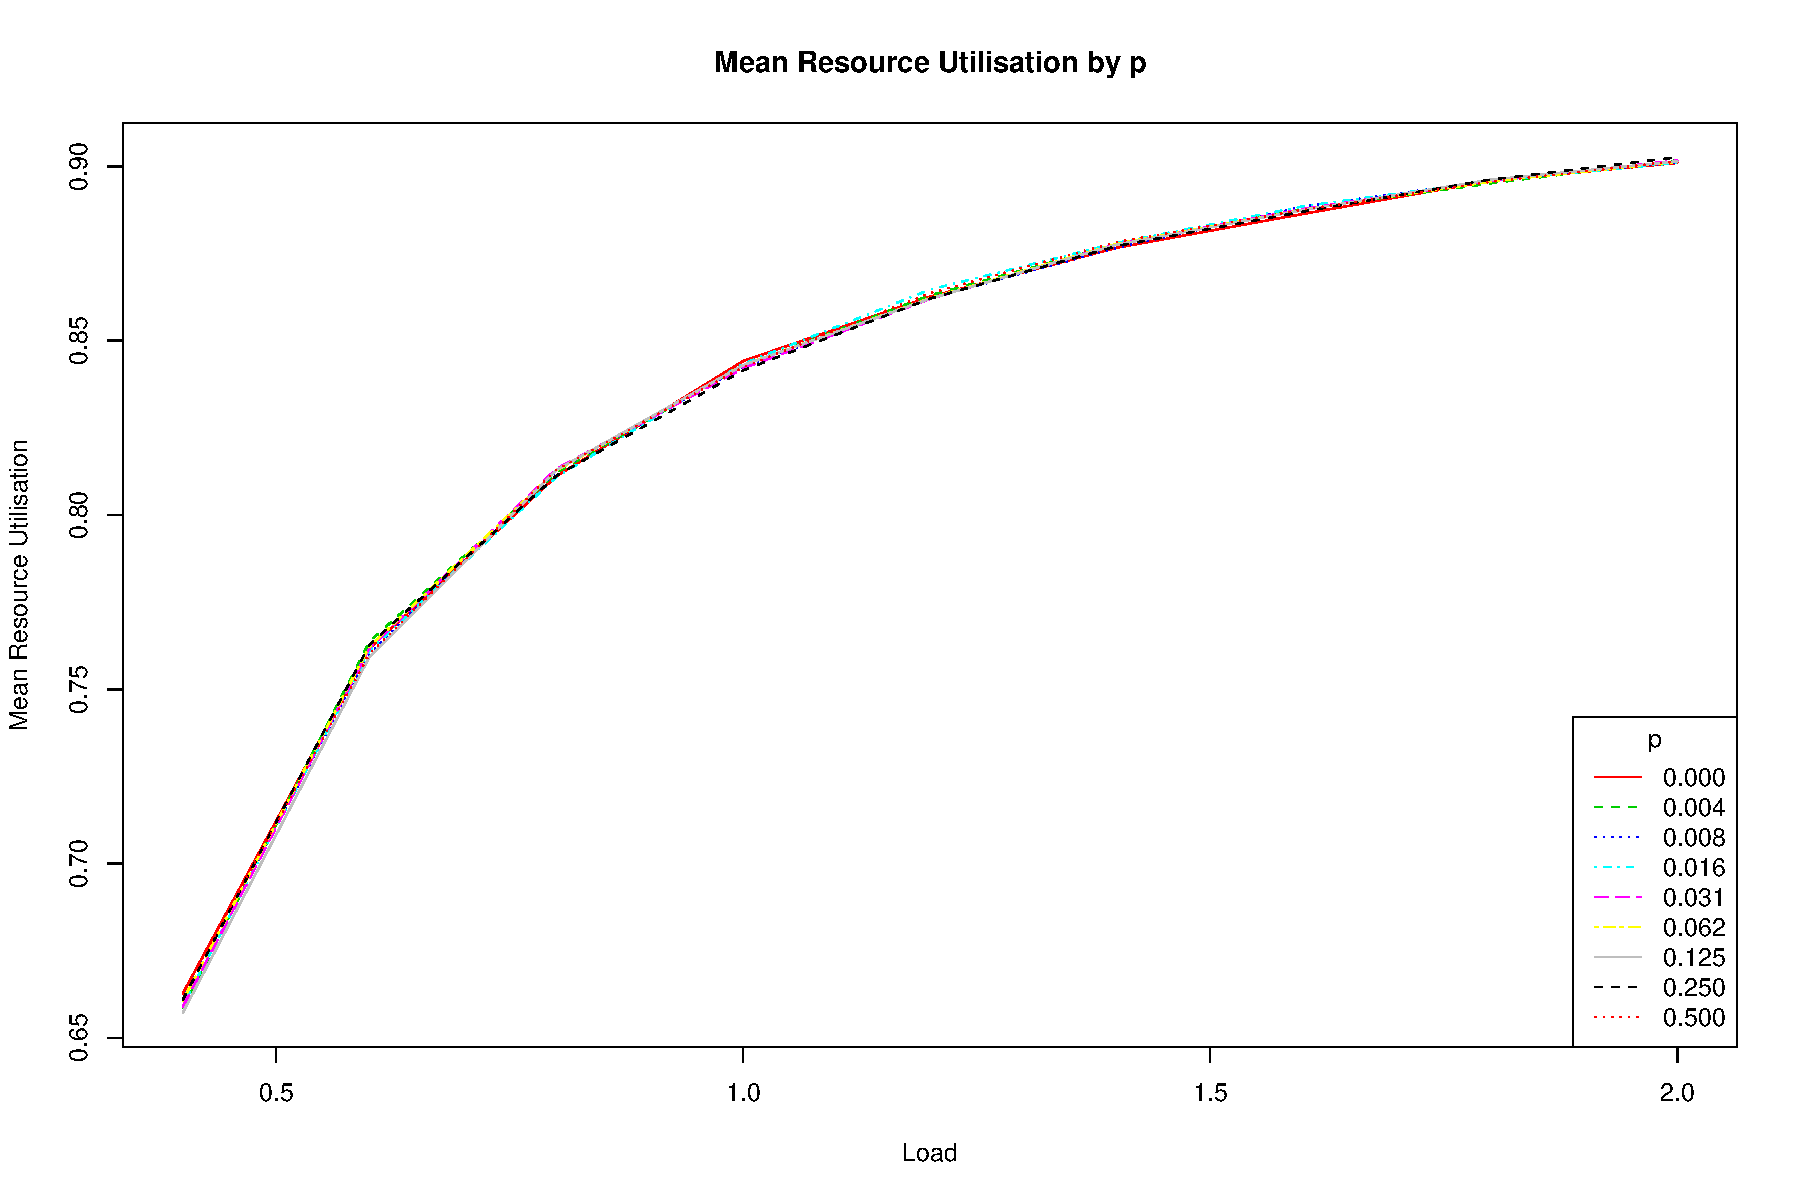
\includegraphics[width=14cm]{images/sw/resource_util_mean}}
  \caption{The mean resource utilisation for a variety of small world networks}
  \label{FIG:RES:SWRUTIL}
\end{figure}

\begin{figure}[h] 
  \centering
  \fbox{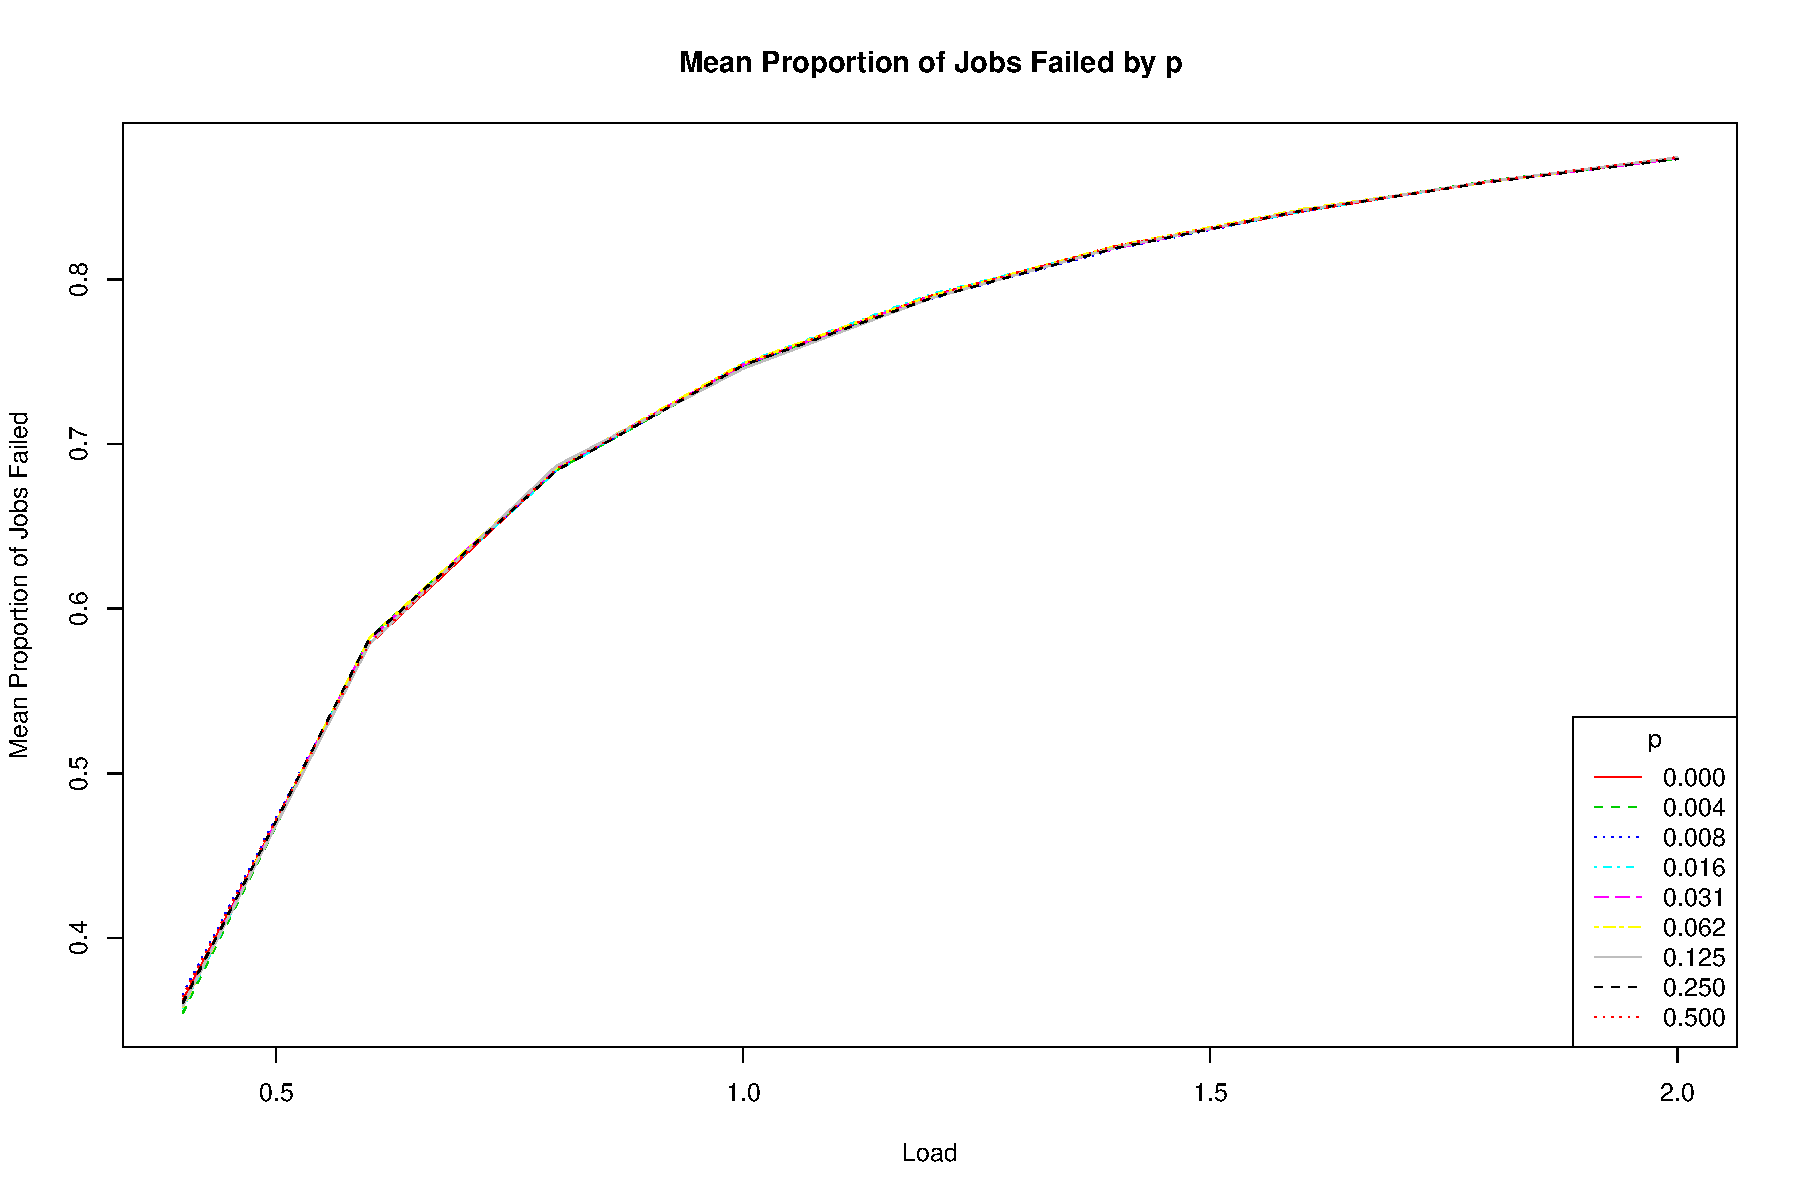
\includegraphics[width=14cm]{images/sw/prop_failed}}
  \caption{The proportion of failed jobs for a variety of small world networks}
  \label{FIG:RES:SWPROPFAILED}
\end{figure}

\begin{figure}[h] 
  \centering
  \fbox{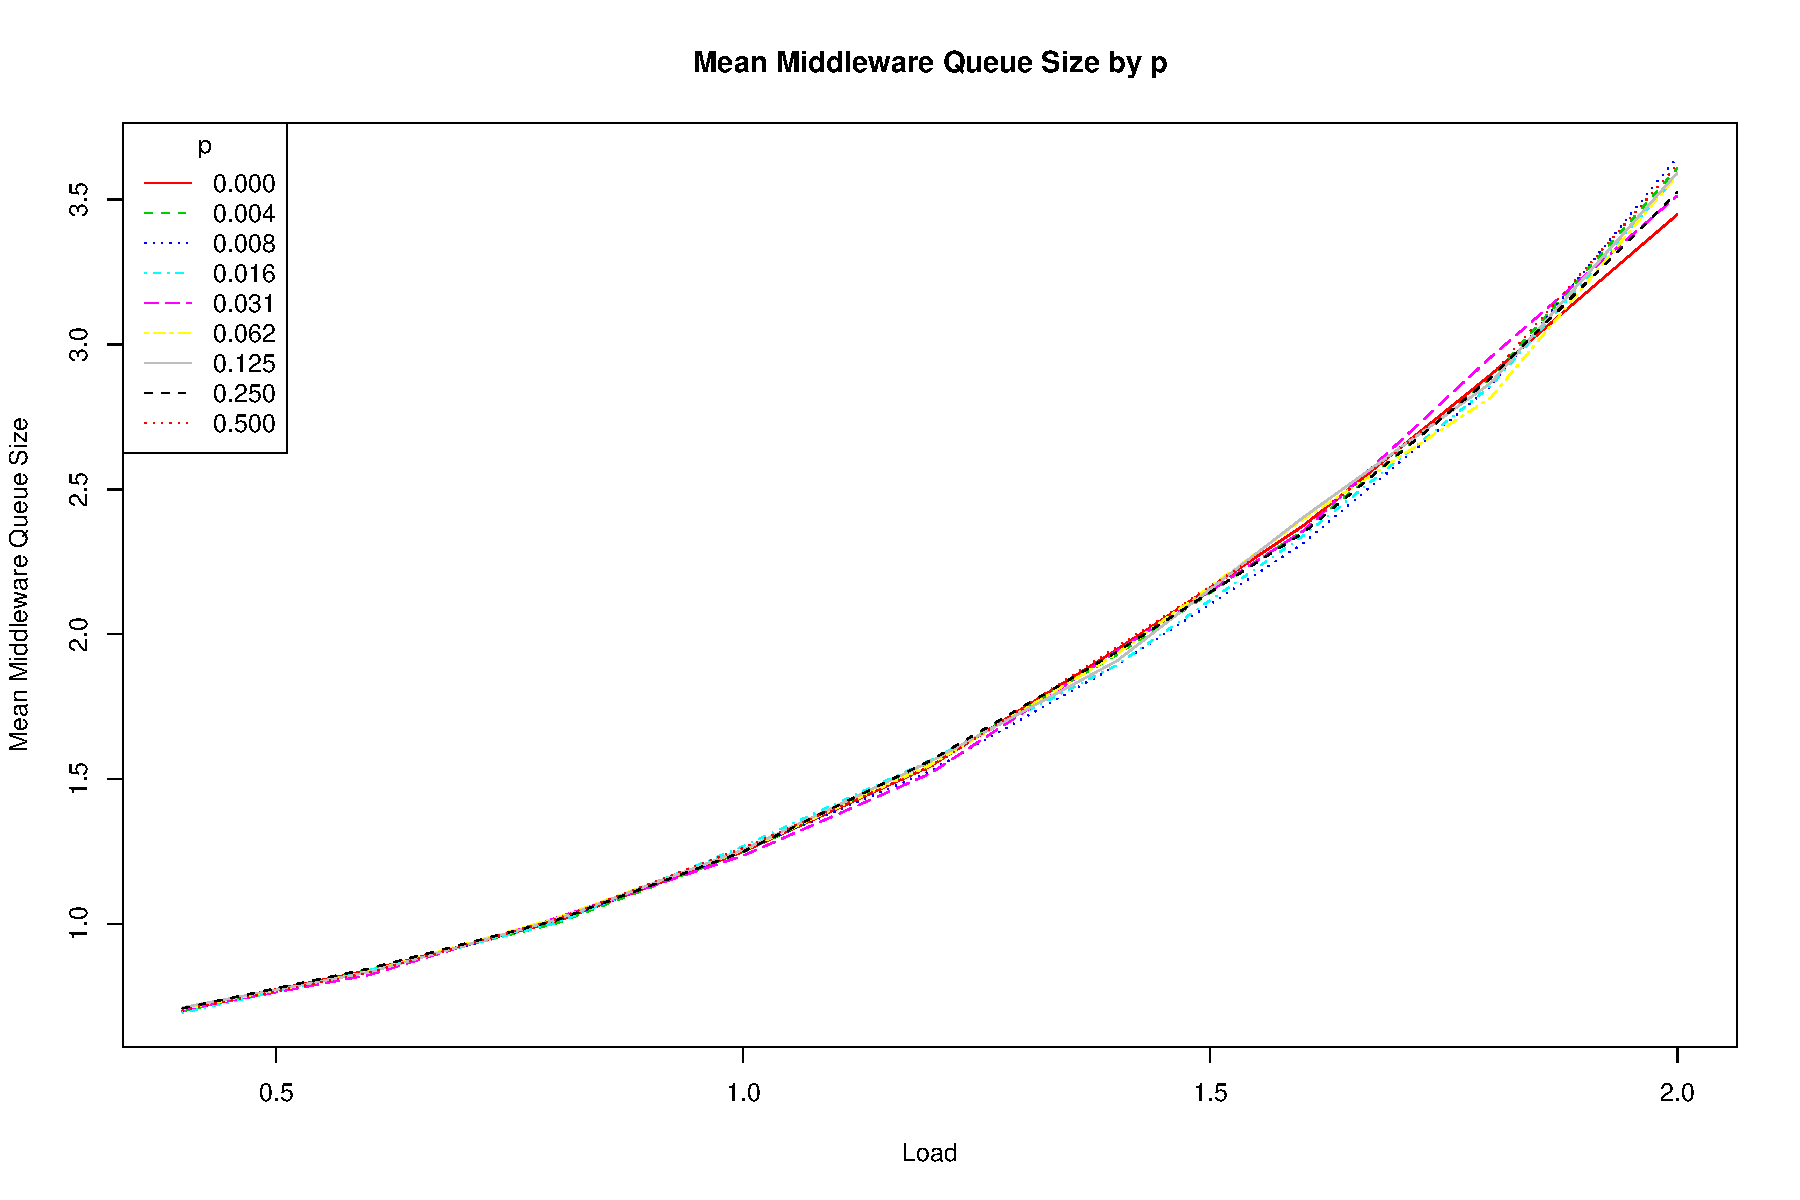
\includegraphics[width=14cm]{images/sw/queue_size_mean}}
  \caption{The mean queue size for a variety of scale-free networks}
  \label{FIG:RES:SFQSIZE}
\end{figure}

\begin{figure}[h] 
  \centering
  \fbox{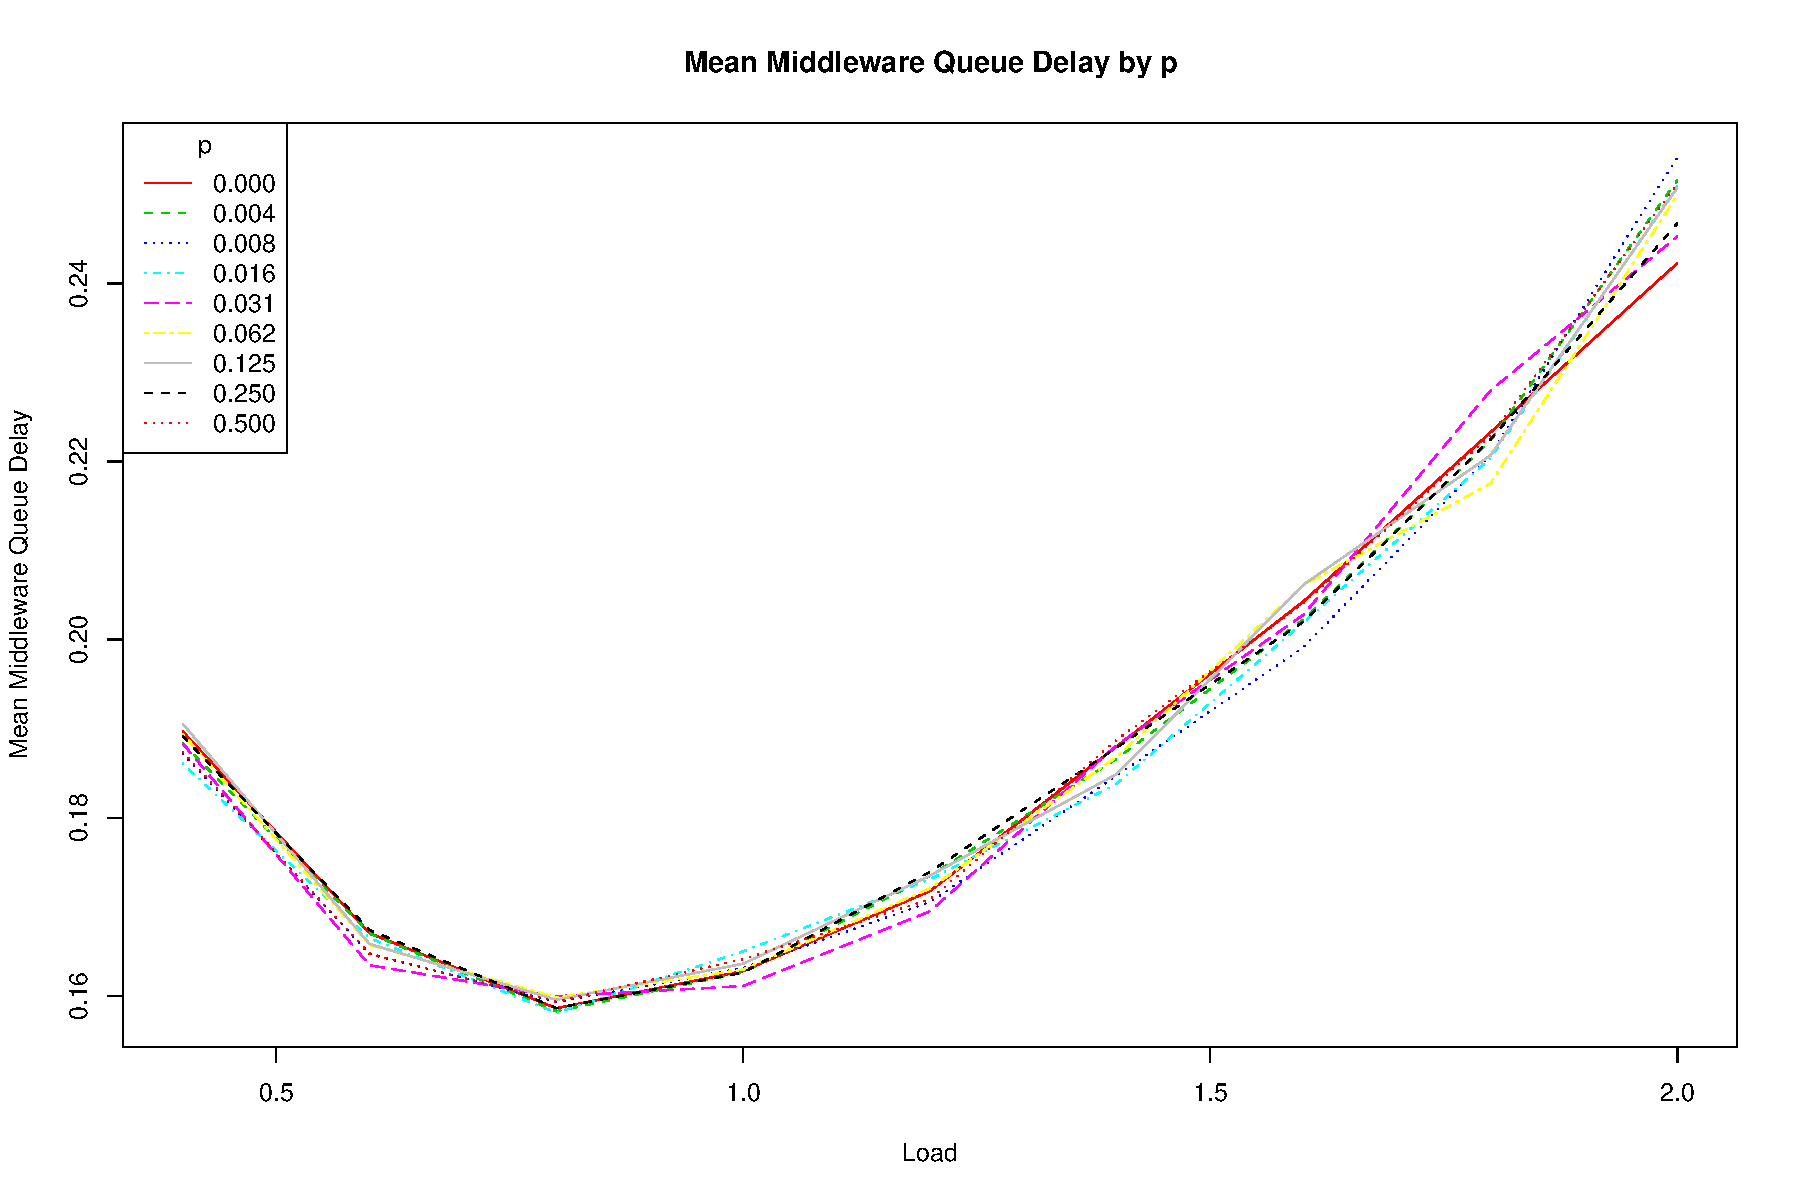
\includegraphics[width=14cm]{images/sw/queue_delay_mean}}
  \caption{The mean queue delay for a variety of scale-free networks}
  \label{FIG:RES:SFQDELAY}
\end{figure}


A variety of small world networks were examined with proportion of global to
local links in the range  $0, \frac{1}{256}, \frac{1}{128}, \frac{1}{64},
\frac{1}{32}, \frac{1}{16}, \frac{1}{8}, \frac{1}{4}, \frac{1}{2}$. The
variation of the proportion made little difference to the performance of the
system as figures \ref{FIG:RES:SWRUTIL} and \ref{FIG:RES:SWPROPFAILED} show.

The scale-free network was examined over a range of value for preferential
treatment. Again the value used made little difference to the performance, with
the exception of a high preference (and thus highly skewed degree distribution)
resulted in queue size and delay, as shown in figures \ref{FIG:RES:SFQSIZE} and
\ref{FIG:RES:SFQDELAY}.  This is likely due the fact that some highly connected
node will struggle to handle the load and build up large queues.

Overall, the different topologies have little impact on the performance of the
system.


